\section{Pulsars and \Acptitle{PWN}}
\seclabel{pulsars_and_pwn}

\subsection{Pulsars}

It is widely accepted that in the collapse of a massive star, a large
amount of ejecta is released as a supernova powering a \ac{SNR}
and that much of the remaining mass collapses into a neutron star
\citep{baade_1934a_remarks-super-novae}.

Pulsars were first discovered observationally in 1967 by Jocelyn Bell
Burnell and Antony Hewish \citep{hewish_1968_observation-rapidly}. They
had constructed a radio telescope that used interplanetary scintillation
with the intention of observing quasars.  In the process, they
detected a source with a periodicity of 1.3 \second. We note in
passing that pulsars had been previously observed by the air force
\citep{brumfiel_2007_force-early}.

Even before the discovery, \cite{pacini_1967_energy-emission}
had predicted the existence of \acp{NS}.  Shortly following
the 1967 discovery, \cite{gold_1968_rotating-neutron} and
\cite{pacini_1968_rotating-neutron} argued that the observed pulsar was
a rotating \ac{NS}.

The discovery of many more pulsars came quickly.  In 1968, and the
Vela pulsar \citep{large_1968_pulsar-supernova} and the Crab pulsar
\citep{staelin_1968_pulsating-radio} were discovered.

The first pulsar observed at optical frequencies was the
Crab, discovered in 1969 shortly after its radio discovery
\citep{cocke_1969_discovery-optical}.  In the same year, the first X-ray
pulsations were discovered from the same source. At the time, there were
no space-based X-ray observatories, so observations had to be performed
from rockets.  The discovery was carried out almost concurrently by
a group at \gls{NRL} \citep{fritz_1969_x-ray-pulsar} and at \gls{MIT}
\citep{bradt_1969_x-ray-optical}.  Using proportional counters, these
experiments showed that the pulsed emission from the Crab extended to
X-ray energies and that, for this source, the X-rays emission was a
factor $>100$ more energetic than the observed visible emission.

From these early sources, pulsar physics has blossomed into a vast
field. In the on-line \ac{ATNF} catalog, there are currently over 2,200
pulsars \citep{manchester_2005a_australia-telescope}.

As was discussed in \secref{history_gamma_ray_detectors},
the first pulsar was observed in $\gamma$-ray in 1970
\citep{kniffen_1970_study-gamma}.  Observations by \ac{EGRET}
brought the total number of $\gamma$-ray-detected pulsars to six
\citep{nolan_1996a_egret-observations}.  \fermi has vastly expanded the
number of pulsars detected in $\gamma$-rays and we will discuss these
observations in \subsecref{2pc}

\subsection{\Acptitle{PWN}}
\subseclabel{pwn}

A \gls{PWN} is a diffuse nebula of shocked relativistic particles
that surrounds and is powered by an accompanying pulsar. 
\glspl{PWN} have been observed long before the discovery of pulsars, but
the pulsar/\gls{PWN} connection was not made until
after the detection of pulsars.

The most famous \glspl{PWN} is the Crab nebula, associated with the Crab
pulsar.  The Crab \ac{SN} (SN 1054), which was observed by Chinese astrologers 
in 1054 AD \cite{hester_2008_nebula:-astrophysical}.
It was also likely observed in
Japan, Europe, by Native Americans,
and in the Arab world 
\citep[see][and references therein]{collins_1999a_reinterpretation-historical}.

\begin{figure}[htbp]
  \centering
  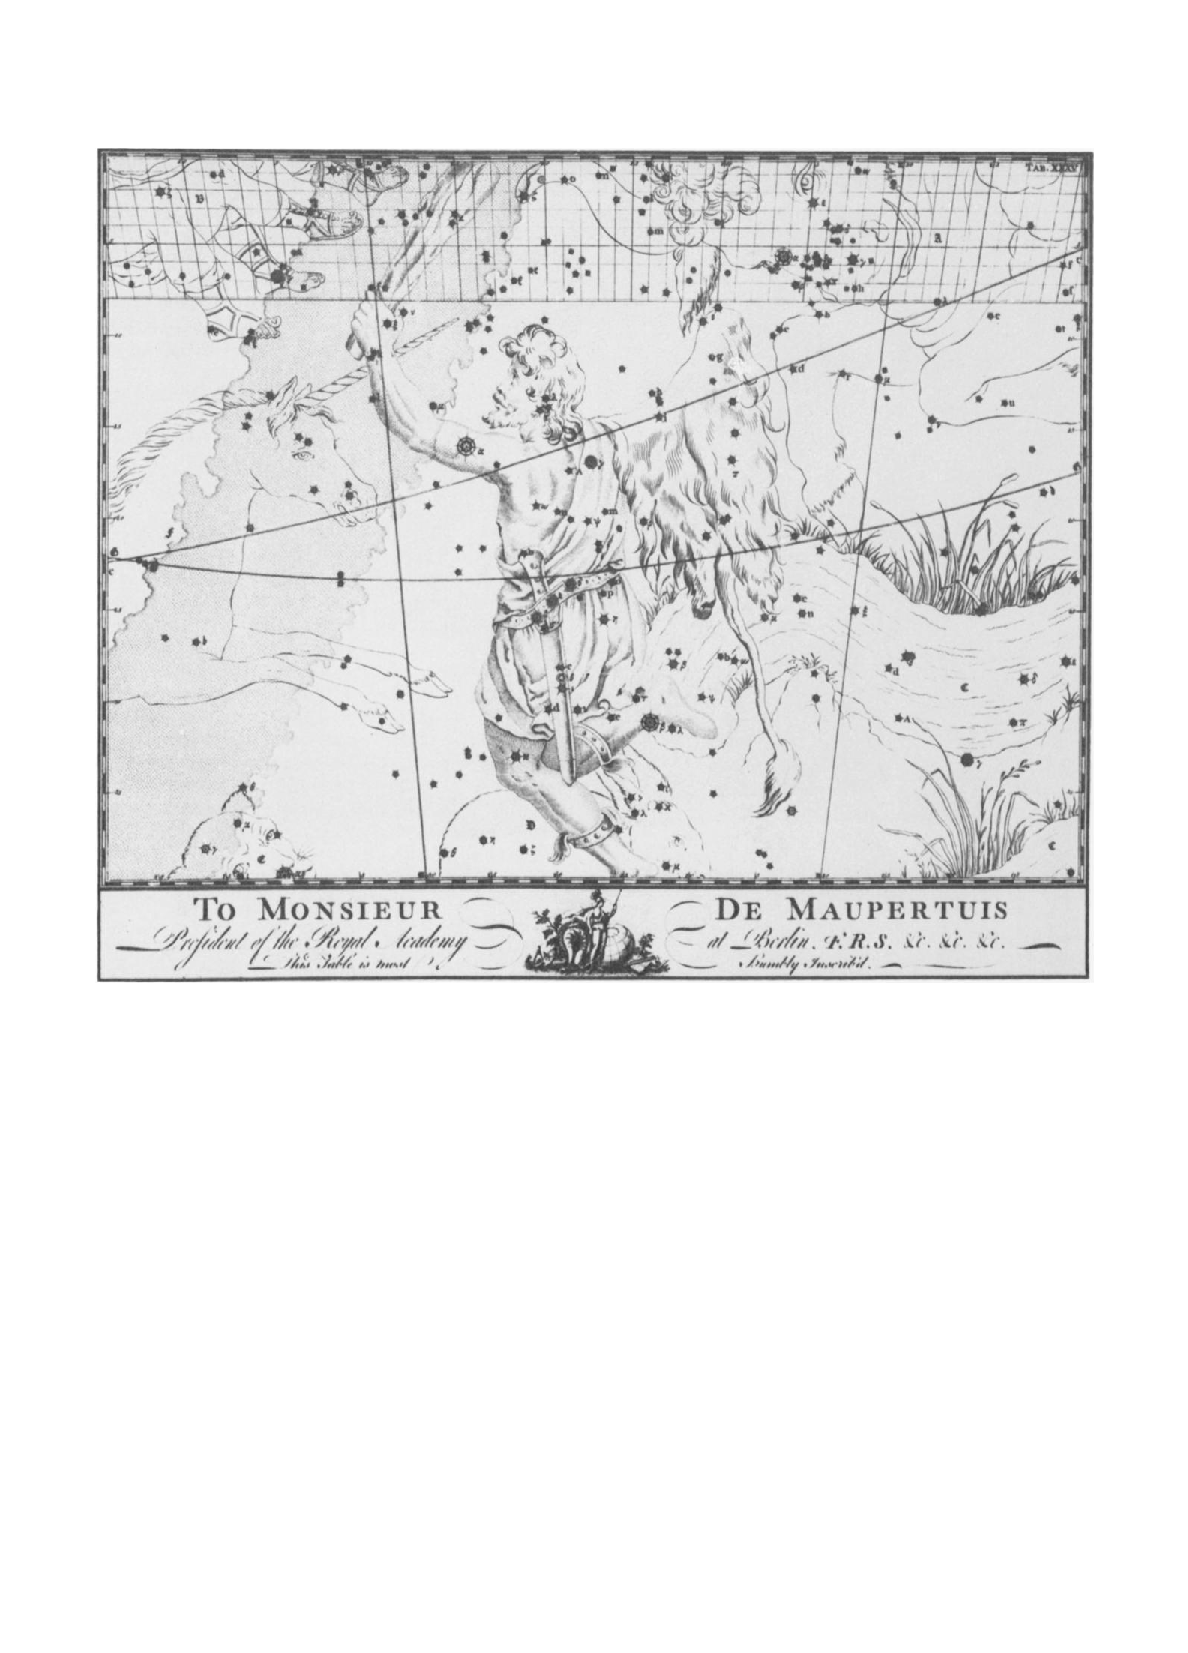
\includegraphics[width=\textwidth]{chapters/introduction/figures/bevis_crab.pdf}
  \figlabel{bevis_crab}
  \caption{The Orion plate from Bevis' book {\em Uranographia Britannica}.
  The Crab nebula can be found on the horn of Taurus the Bull 
  on the top of the figure and the source is marked by a 
  cloudy symbol.
  This figure was reproduced from \cite{ashworth_1981_bevis-uranographia}.}
\end{figure}

The Crab nebula, in the remains of SN 1054,
was first discovered in 1731 by physician and amateur astronomer
John Bevis.  This source was going to be published in his sky atlas
{\em Uranographia Britannica}, but the work was never published because
his published filed for bankruptcy in 1950.  Figure~\figref{bevis_crab}
shows Beavis' plate containing the Crab nebula.  A detailed history of
John Bevis' work can be found in \cite{ashworth_1981_bevis-uranographia}.
The Crab Nebulae was famously included in Charles Messier's catalog as
M1 in 1758 \cite{hester_2008_nebula:-astrophysical}.

In 1921, \cite{lampland_1921a_observed-changes} 
observed motions and changes in brightness of parts of the nebula.
In the same year, \cite{duncan_1921a_changes-observed} observed
that the entire nebula was expanding. Also in the same year
Knut Lundmark proposed a connection between the Crab Nebula
and the 1054 supernova \citep{lundmark_1921a_suspected-stars}
In 1942, \cite{mayall_1942a_further-bearing} connected improved
historical observations with a detailed study of the historical record
to unmistakably connect the Crab nebulae to SN 1054.

Radio emission from the Crab nebula was first detected
in 1949 \citep{bolton_1949a_positions-three}.  The
synchrotron hypothesis for the observed emission was
first proposed by \cite{shklovskii_1953a_nature-nebulas},
and quickly confirmed by optical polarization observations
\citep{dombrovsky_1954a_nature-radiation}.  X-rays from the object were
first detected in \cite{bowyer_1964a_lunar-occultation}.  As was discus
As was discussed in \secref{history_gamma_ray_detectors}, the Crab pulsar
was first detected in \cite{browning_1971_detection-pulsed}.

As was discussed in \secref{history_gamma_ray_detectors}, the Crab pulsar
was discovered in 1968.  In the discovery paper, the \ac{SN}, \ac{PWN},
\ac{NS} connection was proposed \citep{staelin_1968_pulsating-radio}.

The synchrotron and \ac{IC} model of the Crab nebula predicting \ac{VHE}
emission was first proposed by \cite{gould_1965a_energy-cosmic},
and improved in \cite{rieke_1969a_production-cosmic} and
\cite{grindlay_1971a_compton-synchrotron-spectrum}.  As was discussed
in \secref{history_gamma_ray_detectors}, $\gamma$-rays from the Crab
nebula were first observed in \cite{nolan_1993a_observations-pulsar}.
\ac{VHE} emission from the Crab nebula by an \ac{IACT} was first observed
by \cite{weekes_1989a_observation-gamma}.

\acp{PWN} are commonly observed to surround pulsars.
Some of the famous \acp{PWN} include \velax surrounding the Vela
pulsar \citep[first observed in][]{rishbeth_1958a_radio-emission},
\threecfiftyeight \citep{slane_2004a_constraints-structure},
and \mshfifteenfiftytwo \citep{seward_1982a_x-ray-pulsar}.
There are now over 50 sources are identified as being \acp{PWN}
both inside our galaxy in and in the \ac{LMC}
\cite{kaspi_2006_isolated-neutron}.
Many \ac{PWN} have been detected at \ac{VHE} energies.
As of April 2013, the \tevcat\footnote{\tevcat 
is a catalog of \ac{VHE} sources compiled by the University of
Chicago. It can be found at \url{http://tevcat.uchicago.edu}.} 
includes 31 \ac{VHE} sources classified as \acp{PWN}.
We will discuss these \ac{VHE} \ac{PWN} in \chapref{tevcat}.
